\documentclass[9pt]{beamer}

% apparence
\usetheme{Singapore}
\usecolortheme{orchid}
\setbeamercolor{title}{
    use=structure,fg=white,bg=structure.fg!75!black
}
\useinnertheme[shadow]{rounded}

% numéro des slides
\addtobeamertemplate{navigation symbols}{}{
    \usebeamerfont{footline}
    \usebeamercolor[fg]{footline}
    \hspace{1em}
    \raisebox{2pt}{
        \insertframenumber/\inserttotalframenumber
    }
}

% réduire l'espace sous les titres de slides
\addtobeamertemplate{frametitle}{}{\vspace*{-5mm}}

\makeatletter

% afficher/masquer dans miniframes
\let\beamer@writeslidentry@miniframeson=\beamer@writeslidentry
\def\beamer@writeslidentry@miniframesoff{
    \expandafter\beamer@ifempty\expandafter{\beamer@framestartpage}{}
    {\clearpage\beamer@notesactions}
}

\newcommand*{\miniframeson}{
    \let\beamer@writeslidentry=\beamer@writeslidentry@miniframeson
}

\newcommand*{\miniframesoff}{
    \let\beamer@writeslidentry=\beamer@writeslidentry@miniframesoff
}

% séparation épaisse dans un tableau
\def\hlinewd#1{
\noalign{\ifnum0=`}\fi\hrule \@height #1
\futurelet\reserved@a\@xhline}

\makeatother

% packages
\usepackage{graphicx, multirow}
\usepackage{algorithm, algpseudocode}
\usepackage[dvipsnames]{xcolor}

% titre du beamer
\title{Adaptive Kriging Particle Filter and its Application to Terrain-Aided Navigation}

\author{Bastien HUBERT\inst{1, 2}, Karim DAHIA\inst{1},\\Nicolas MERLINGE\inst{1}, Audrey GIREMUS\inst{2}}

\institute{\inst{1} ONERA, DTIS, IGNC\quad\inst{2} Université de Bordeaux, CNRS, IMS}

\date{}

\titlegraphic{
\vspace{-\baselineskip}

\includegraphics[width=10cm]{../../Images/Logo ONERA IMS.pdf}
}

% début du beamer
\begin{document}

\begin{frame}
\begin{center}
\includegraphics[width=3cm]{../../Images/Logo FUSION 2024.png}
\hspace{1cm}
\raisebox{10pt}{\includegraphics[width=2cm]{../../Images/Logo IEEE.png}}
\vspace{-\baselineskip}
\end{center}

\titlepage

\end{frame}

\logo{
\includegraphics[width=1.5cm]{../../Images/Logo FUSION 2024.png}
\hspace{2mm}
\raisebox{5pt}{\includegraphics[width=1cm]{../../Images/Logo IEEE.png}}
\hspace{4.5cm}

\includegraphics[width=5cm]{../../Images/Logo ONERA IMS.pdf}}

\section{Introduction}

\begin{frame}{Context: autonomous navigation for UAVs}

\begin{block}{Inertial navigation for Unmanned aerial vehicles (UAVs)}
\begin{itemize}
\item Integrates measurements from the accelerometers and gyrometers of an inertial measurement unit (IMU)
\item Autonomous and reliable on short missions
\item But imperfect measures (biases, scale factors, noises, ...)
\item[$\Rightarrow$] Drifts over time
\end{itemize}
\end{block}

\begin{block}{Data fusion}
\begin{itemize}
\item Using data from other sensors helps reduce the drift
\item GNSS as an ideal counterpart to inertial data, but not always available
\item[$\Rightarrow$] Physical field-aided navigation instead
\item Measures from exteroceptive onboard sensors
\item Comparison between the measured data and an embedded map
\end{itemize}
\end{block}

\end{frame}

\begin{frame}{Case of study: Terrain aided-navigation (TAN)}

\begin{columns}[onlytextwidth]

\begin{column}{0.4\textwidth}
\begin{center}
\hspace{-5mm}
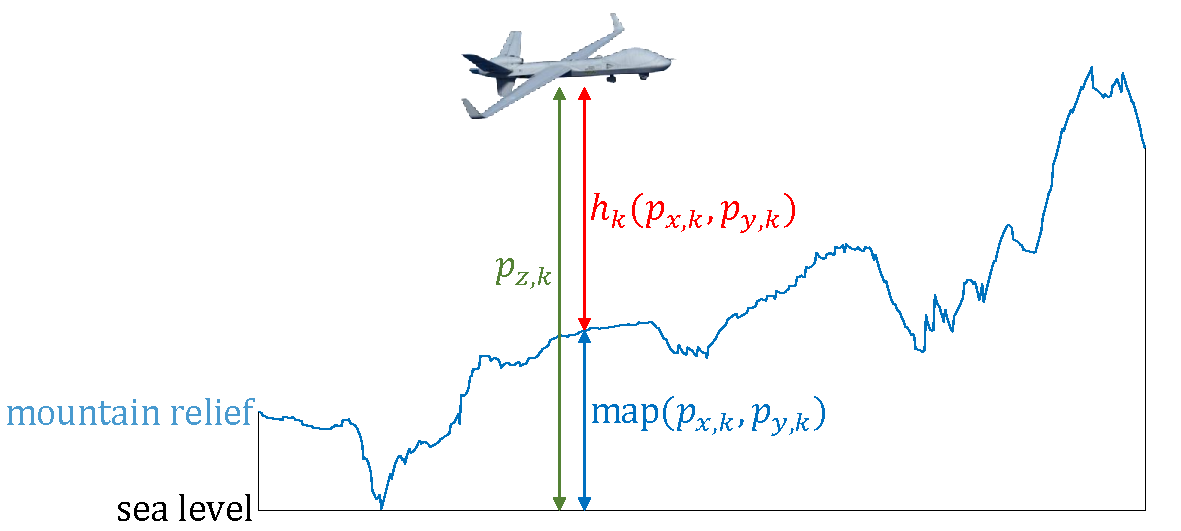
\includegraphics[width=\textwidth]{../../Images/Schéma de la corrélation de terrain.pdf}
\end{center}
\end{column}

\begin{column}{0.55\textwidth}
\begin{block}{Terrain-aided navigation}
\begin{itemize}
\item Measurement of the overflown terrain altitude by a radar-altimeter
\item Comparison with an embedded map
\end{itemize}
\end{block}
\end{column}

\end{columns}

\vspace{2.5mm}

\begin{columns}

\begin{column}{0.5\textwidth}
\begin{block}{Challenges}
\begin{itemize}
\item High initial state uncertainty
\item Ambiguous and non-analytical environment model
\item Poorly-known environment:
\begin{itemize}
\item Noisy and under-sampled field
\item Better map too big to embed
\end{itemize}
\end{itemize}
\end{block}
\end{column}

\begin{column}{0.45\textwidth}
\begin{center}
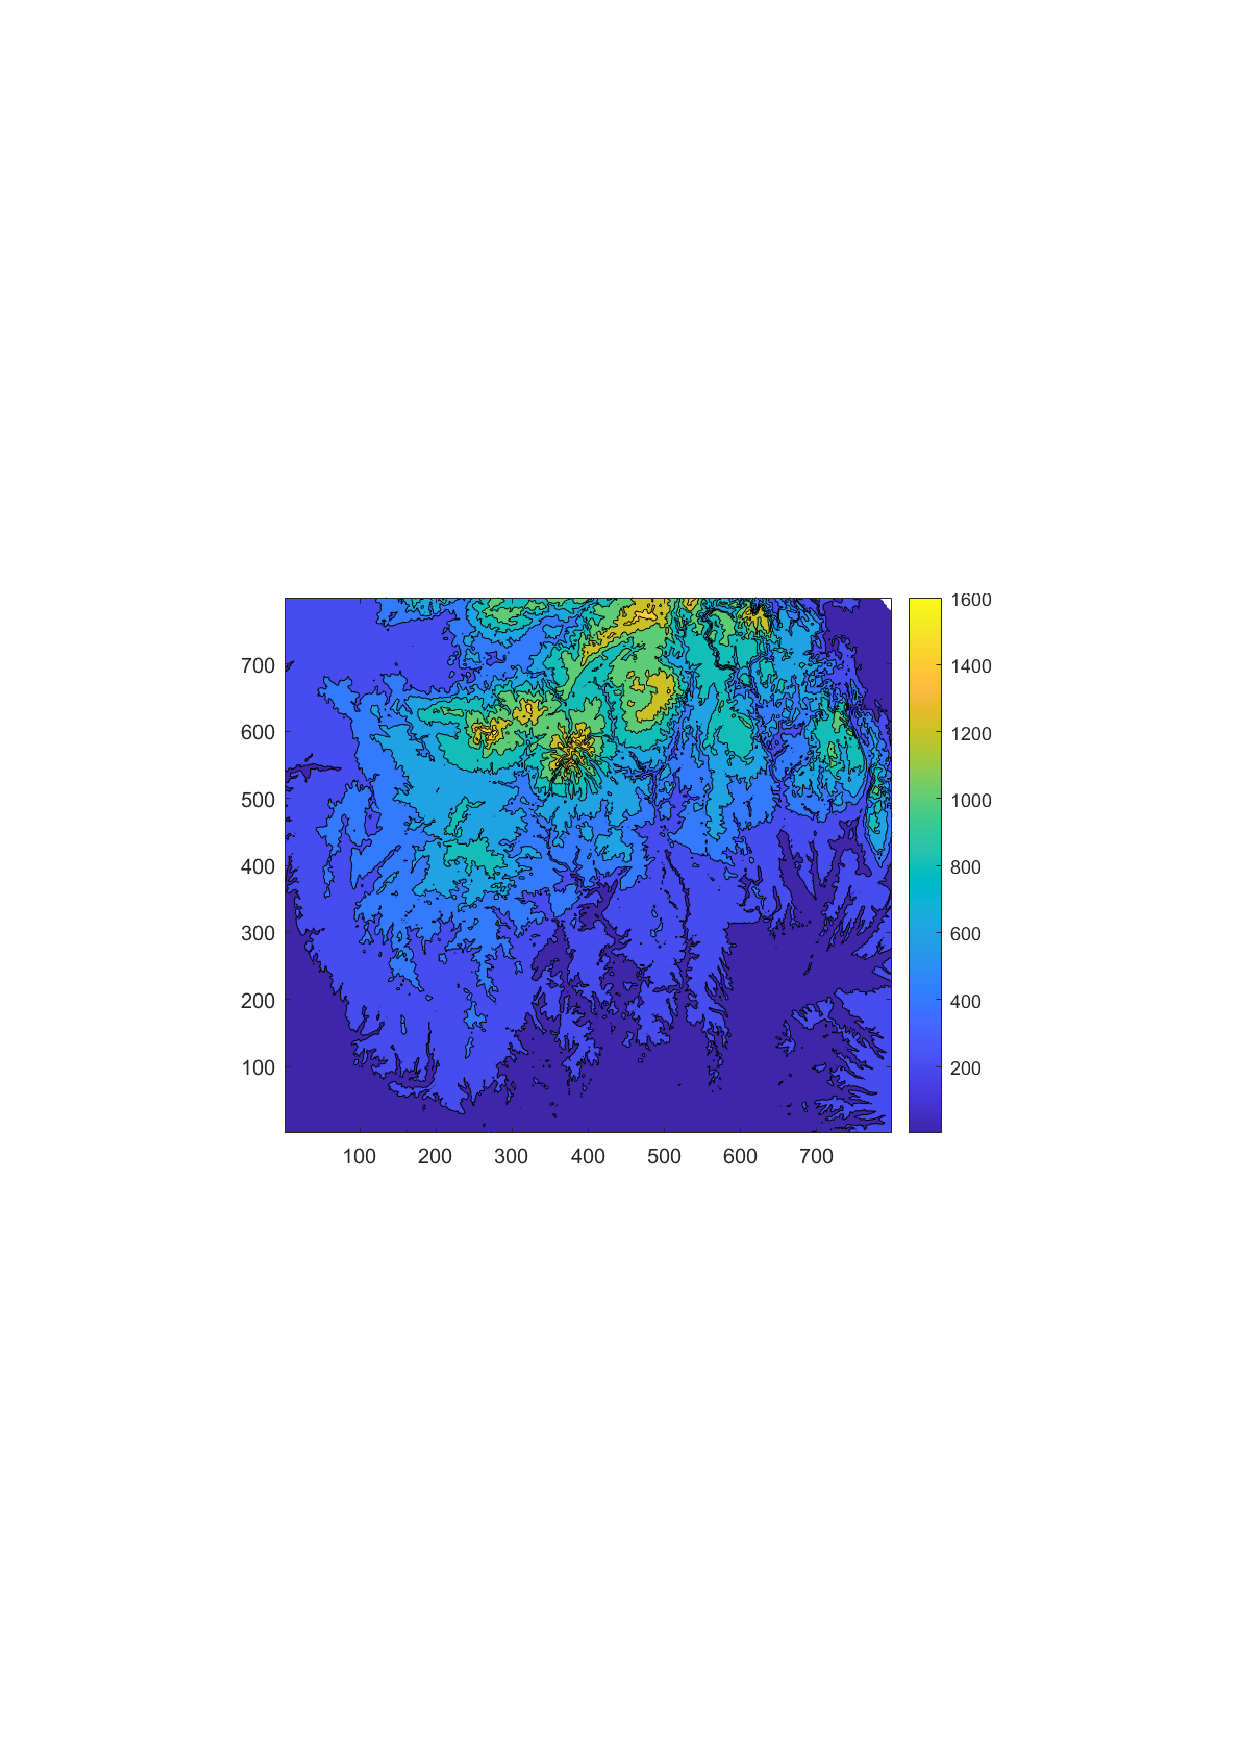
\includegraphics[width=\textwidth]{../../Images/Carte altimétrique FUSION 2024.pdf}
\end{center}
\end{column}

\end{columns}

\end{frame}

\section{Problem statement}

\begin{frame}{Bayesian estimation}

\begin{block}{Discrete state-space representation}
\begin{itemize}
\item \hfill $\left\{
\begin{aligned}
x_k & = \mathcal{F}_k(x_{k-1}, \nu_k) & \text{recursive dynamical process} \\
z_k & = \mathcal{H}_k(x_k) + \eta_k & \text{measurement equation}
\end{aligned}
\right.$ \hfill (1)
\end{itemize}
\end{block}

\begin{block}{Bayesian filtering}
\begin{itemize}
\item Goal: compute $p(x_k|z_{1:k})$ the posterior probability density function (PDF)
\item State estimation:\\
\hfill $\displaystyle \hat x_k^{EAP} = \mathbb{E}(x_k|z_{1:k}) = \int x_k \: p(x_k|z_{1:k}) \: dx_k$ \hfill (2)
\item Error covariance matrix:\\
\hfill $\displaystyle P_k^{EAP} \triangleq \mathbb{V}(\hat{x}_k^{EAP}) = \int (x_k - \hat{x}_k^{EAP})(x_k - \hat{x}_k^{EAP})^T p(x_k|z_{1:k}) \: dx_k$ \hfill (3)
\end{itemize}
\end{block}

\end{frame}

\begin{frame}{Bayesian estimation}

\begin{block}{Optimal Bayesian filter}
\begin{itemize}
\item Recursive process in two steps:
\begin{itemize}
\item Prediction step with Chapman-Kolmogorov's equation:\\
\hfill $\displaystyle p(x_k|z_{1:k-1}) = \underbrace{\int p(x_k|x_{k-1}) \: p(x_{k-1}|z_{1:k-1}) \: dx_{k-1}}_{\text{no analytical solution}}$ \hfill (4)
\item Correction step with Bayes' formula:\\
\hfill $\displaystyle p(x_k|z_{1:k}) = \frac{p(z_k|x_k) \: p(x_k|z_{1:k-1})}{\int p(z_k|x_k) \: p(x_k|z_{1:k-1}) \: dx_k}$ \hfill (5)
\end{itemize}
\end{itemize}
\end{block}

\begin{columns}[onlytextwidth]

\begin{column}{0.55\textwidth}
\begin{block}{Kalman filter}
\begin{itemize}
\item Optimal analytical estimation under strong assumptions:
\begin{itemize}
\item Linear equations and Gaussian noises
\end{itemize}
\item Poorly handles ambiguities and multi-modality
\item[$\Rightarrow$] Stochastic methods are superior in these cases
\end{itemize}
\end{block}

\end{column}

\begin{column}{0.4\textwidth}
\begin{center}
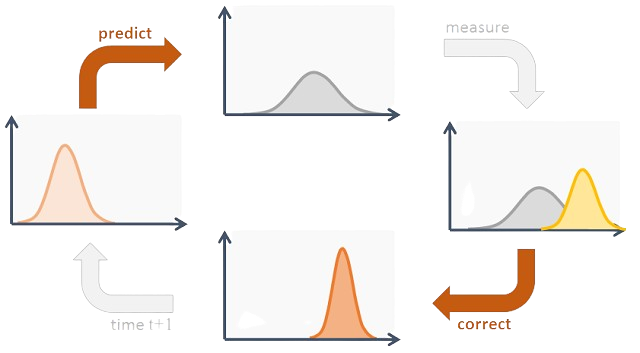
\includegraphics[width=\textwidth]{../../Images/Étapes du filtre de Kalman avec images.png}
\end{center}
\end{column}

\end{columns}

\end{frame}

\begin{frame}{Particle filtering}

\begin{block}{Standard particle filter}
\begin{itemize}
\item Importance sampling method
\item Asymptotically optimal with weak assumptions:
\begin{itemize}
\item $\mathcal{F}_k$, $\mathcal{H}_k$ and noise distributions known
\end{itemize}
\item Posterior PDF approximation using a mixture of Dirac distributions:\\
\hfill $\displaystyle p(x_k|z_{1:k}) \approx \sum_{i=1}^{N_p} w_k^i \: \delta\left(x_k-x_k^i\right)$ \hfill (6)
\item Prediction step: $\displaystyle x_k^{(i)} \sim q\left(\cdot\:|x_{k-1}^{(i)},z_k\right)$
\item Correction step: $\displaystyle w_k^{(i)} \propto w_{k-1}^{(i)} \: \frac{p\left(z_k|x_k^{(i)}\right) \: p\left(x_k^{(i)}|x_{k-1}^{(i)}\right)}{q\left(x_k^{(i)}|x_{k-1}^{(i)},z_k\right)}$ \hfill (7)
\item Usual proposal: $\displaystyle q\left(x_k^{(i)}|x_{k-1}^{(i)},z_k\right) = p\left(x_k^{(i)}|x_{k-1}^{(i)}\right)$
\end{itemize}
\end{block}

\end{frame}

\begin{frame}{Regularised particle filter (RPF)}
\vspace*{5mm}

\begin{block}{Regularised particle filter}
\begin{itemize}
\item Particle degeneracy during the correction step $\rightarrow$ resampling if:\\
\hfill $\displaystyle N_{eff} \triangleq \frac{1}{\sum_{i=1}^{N_p}\left(w_k^i\right)^2} <  \alpha_{th} \: N_p \quad \text{with } 0 < \alpha_{th} < 1$ \hfill (8)
\item Particle impoverishment due to duplication $\rightarrow$ regularisation
\item Kernel density approximation of the PDF:
\end{itemize}
\hfill $\displaystyle p(x_k|z_{1:k}) \approx \sum_{i=1}^{N_p} w_k^i \: \mathcal{K}_h\left(x_k-x_k^i\right)$ \hfill (9)
\end{block}

\begin{center}
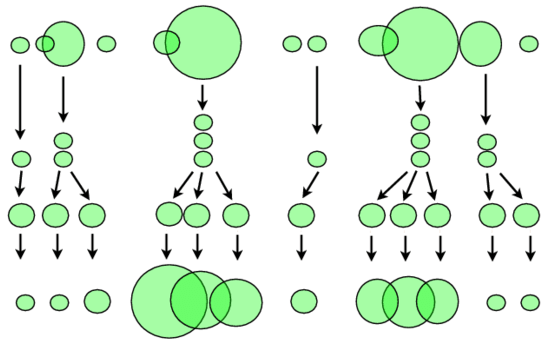
\includegraphics[width=0.5\textwidth]{../../Images/Étapes du RPF.png}
\end{center}

\end{frame}

\section{Adaptive Kriging Particle Filter}

\begin{frame}{Gaussian process regression}
\vspace*{5mm}

\begin{block}{Navigation in Poorly-Known Environment}
\begin{itemize}
\item Poorly-known environment $\rightarrow$ Bayesian correction is impossible
\item Measurement field too complex for multi-linear interpolation
\item[$\Rightarrow$] Kriging grants an analytical expression of the measurement function and noise conditional to some training data
\end{itemize}
\end{block}

\begin{center}
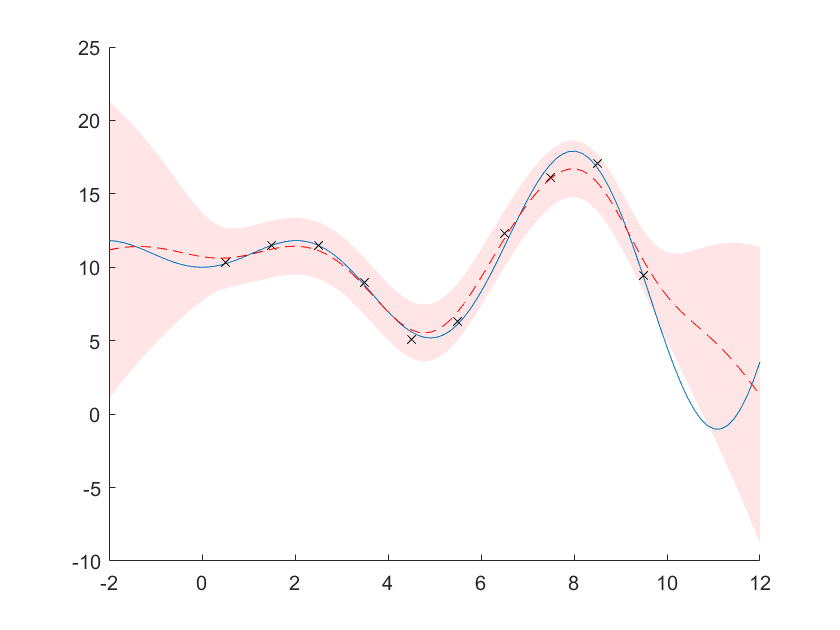
\includegraphics[width=0.6\textwidth]{../../Images/Exemple de krigeage 2D.png}
\end{center}

\end{frame}

\begin{frame}{Gaussian process regression}

\begin{columns}[onlytextwidth]

\begin{column}{0.35\textwidth}

\begin{center}
\hspace*{-10mm}
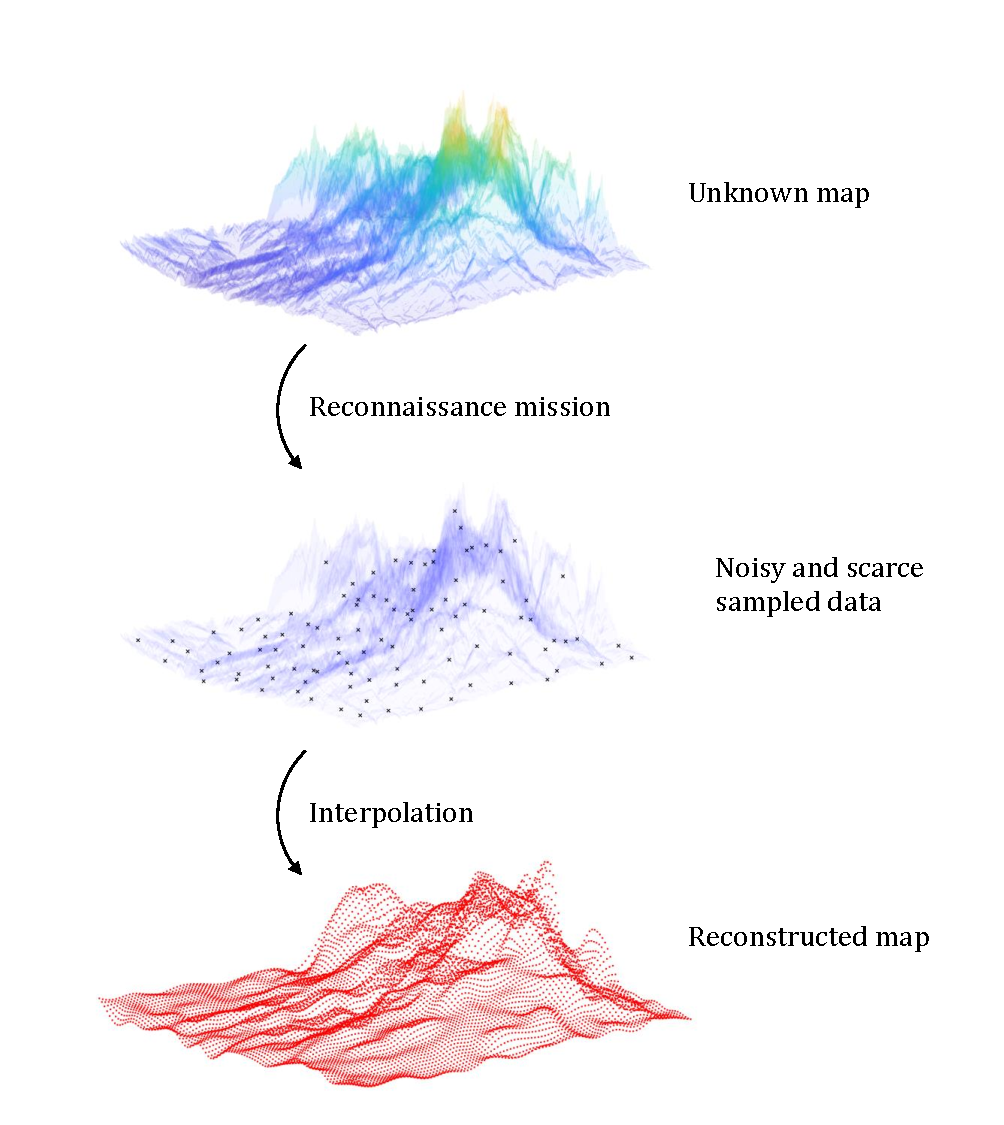
\includegraphics[width=\dimexpr\textwidth+8mm\relax]{../../Images/Étapes du krigeage.pdf}
\end{center}

\end{column}

\begin{column}{0.65\textwidth}

\begin{block}{Gaussian process regression}

\begin{itemize}
\setlength\itemsep{5pt}
\item Particles and training data:\\[5pt]
\hfill \scalebox{0.8}{$\left\{
\begin{matrix}
\forall i \in [\![1, n]\!], & z^i = \mathcal{H}(x^i) + \eta^i & \eta^i \sim(0, R) \\
\forall j \in [\![1, \tilde n]\!], & \tilde z^j = \mathcal{H}(\tilde x^j) + \tilde\eta^j & \tilde\eta^j \sim(0, \tilde R)
\end{matrix}
\right.$} \hfill (18)
\item Conditional probability distribution:\\[5pt]
\hfill \scalebox{0.8}{$z|\tilde z \sim \mathcal{N}(\mu^*(x, \tilde{x}, \tilde{z}), R^*(x, \tilde{x}))$} \hfill \mbox{}\\[5pt]
\hfill \scalebox{0.8}{$\left\{
\begin{aligned}
A(x, \tilde{x}) &  =
\mathcal{K}(x, \tilde{x}) \:
\left(\mathcal{K}(\tilde{x}, \tilde{x}) + I_{\tilde n} \otimes \tilde R\right)^{-1} \\
\mu^*(x, \tilde{x}, \tilde{z}) & =
\mu(x) + A(x, \tilde{x}) \:
(\tilde{z} - \mu(\tilde{x})) \\
R^*(x, \tilde{x}) & =
\mathcal{K}(x, x) +
I_n \otimes R -
A(x, \tilde{x}) \:
\mathcal{K}(x, \tilde{x})^T
\end{aligned}
\right.$} \hfill (20)
\item Kriged measurement function:\\[5pt]
\hfill \scalebox{0.8}{$\begin{matrix}
z_k = \mu^*(x_k, \tilde{x}, \tilde{z}) + \eta^*_k & \eta^*_k \sim(0, R^*(x_k, \tilde{x}))
\end{matrix}$} \hfill (21)
\end{itemize}
\end{block}

\end{column}

\end{columns}

\end{frame}

\begin{frame}{Adaptive kriging (AK)}

\begin{block}{Fitting the model}
\begin{itemize}
\item Chosen GP: $\mu:x\mapsto \mu_0$ and $\mathcal{K}:x, x'\mapsto \sigma_f^2 \: \text{exp}\left(-\frac{1}{2} \frac{(x-x')^T (x-x')}{l^2}\right)$
\item Computation of the hyperparameters by maximum likelihood estimation
\end{itemize}
\end{block}

\begin{columns}[onlytextwidth]

\begin{column}{0.35\textwidth}

\begin{center}
\hspace*{-10mm}
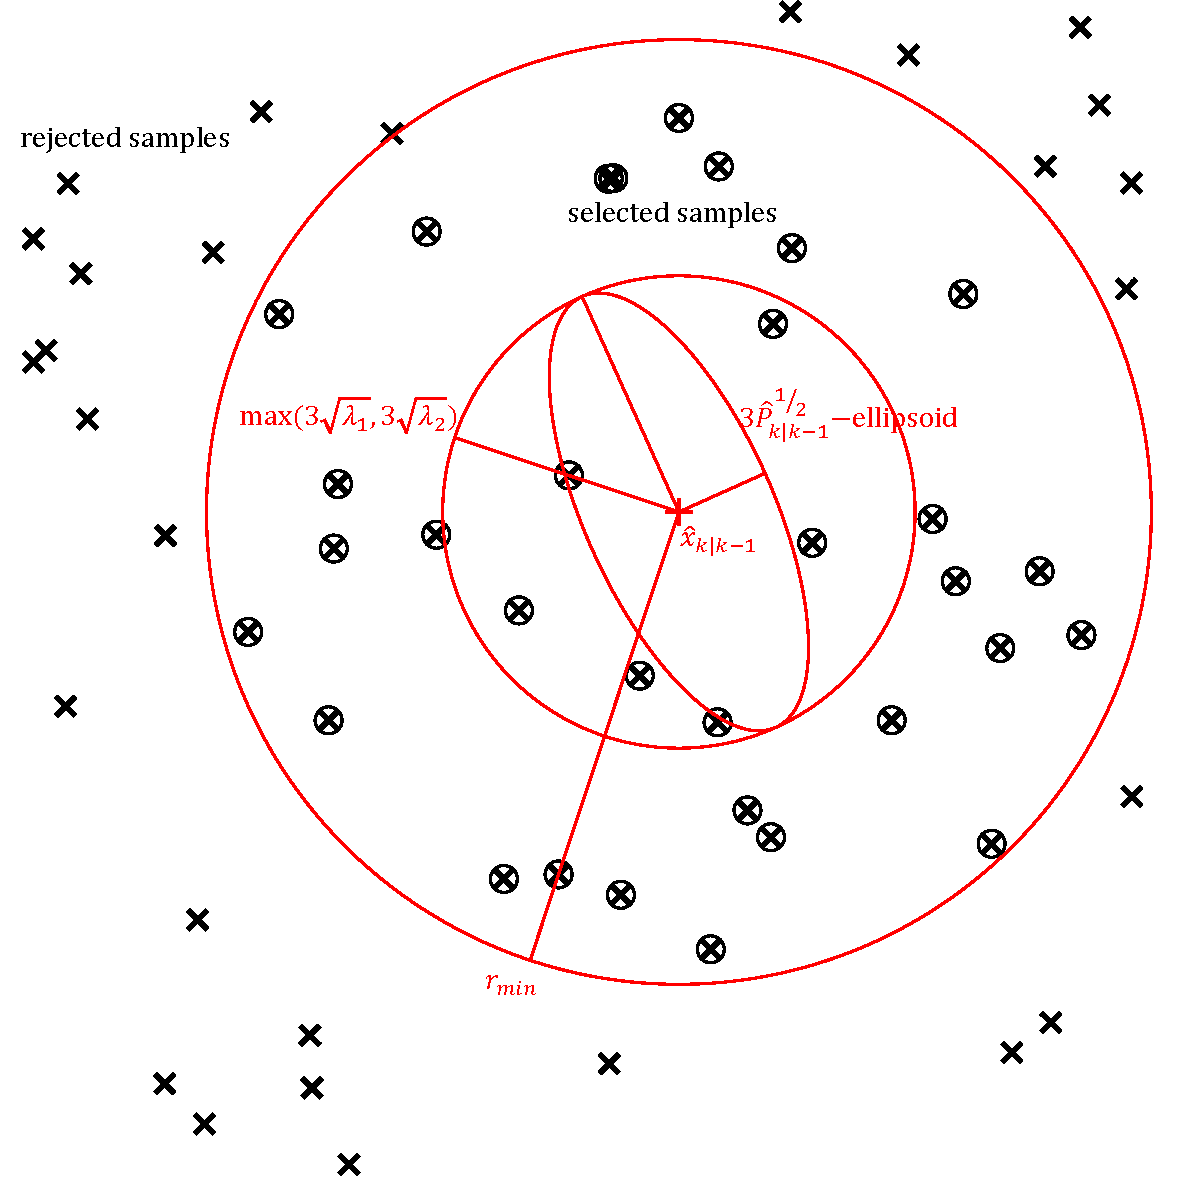
\includegraphics[width=\textwidth]{../../Images/Fenêtrage du krigeage adaptatif.pdf}
\end{center}

\end{column}

\begin{column}{0.65\textwidth}

\begin{block}{Training data selection}
\begin{itemize}
\item Non-stationarity of the correction field
\item Need to select relevant training data
\item Moving window:\\
\hfill \scalebox{0.75}{$W_k \triangleq \{j \in  [\![1, \tilde n]\!] : ||\tilde x^j - \pi_g(\hat x_{k|k-1})||_2 < r_k\}$} \hfill (24)
\item Adaptive radius:\\
\hfill \scalebox{0.75}{$\left\{
\begin{aligned}
r_k & \triangleq \text{min}\{r \in [r_{min,k}, +\infty[ \:: \text{Card}(W_k) \geq N_{W,min}\} \\
r_{min,k} & \triangleq \alpha_W \times \underset{\lambda \in \text{sp}(\pi_g(\hat P_{k|k-1}))}{\text{max}}\left(3\sqrt{\lambda}\right)
\end{aligned}
\right.$} \hfill (25)
\end{itemize}
\end{block}

\end{column}

\end{columns}

\end{frame}

\begin{frame}{AK-RPF pseudo-code}
\begin{block}{Algorithm overview}

\begin{algorithmic}
\algrenewcommand\algorithmicif{if}
\algrenewcommand\algorithmicthen{then}
\algrenewcommand\algorithmicend{end}

\State $\forall i \in [\![1, N_p]\!]$, draw $x_k^i$ from $p(\cdot|x_{k-1}^i)$ \Comment{Prediction}
\State \textcolor{BrickRed}{compute $r_k$ from (25) \Comment{Adaptive selection}}
\State \textcolor{BrickRed}{extract $W_k$ from the training set using (24)}
\State \textcolor{BrickRed}{fit the process to the extracted data by MLE \Comment{Adaptive GP}}
\State \textcolor{BrickRed}{$\forall i \in [\![1, N_p]\!]$, compute $p(z_k|x_k^i)$ according to (20) \Comment{Kriging}}
\State $\forall i \in [\![1, N_p]\!]$, compute $w_k^i$ according to (7) \Comment{Correction}
\State $\hat x_k \gets \sum_{i=1}^{N_p} w_k^i x_k^i$ \Comment{Estimation}
\State $\hat P_k \gets \sum_{i=1}^{N_p} w_k^i (x_k^i - \hat x_k) (x_k^i - \hat x_k)^T$
\If{(8)}
\State resample $\left(x_k^{1:N_p},w_k^{1:N_p}\right)$ \Comment{Resampling}
\State $\forall i \in [\![1, N_p]\!]$, draw $\varepsilon_k^i$ from the regularisation kernel \Comment{Regularisation}
\State $\forall i \in [\![1, N_p]\!], \: x_k^i \gets x_k^i + \alpha_{reg}\:h\:\hat P_k^{\frac{1}{2}}\:\varepsilon_k^i$
\State $\hat x_k \gets \sum_{i=1}^{N_p} w_k^i x_k^i$ \Comment{Re-estimation}
\State $\hat P_k \gets \sum_{i=1}^{N_p} w_k^i (x_k^i - \hat x_k) (x_k^i - \hat x_k)^T$
\EndIf
\end{algorithmic}

\end{block}
\end{frame}

\section{Application to TAN}

\begin{frame}{Simulation}
\begin{block}{Simulation parameters}

\begin{itemize}
\item Uniform rectilinear motion
\item 100 Monte Carlo trials per filter
\end{itemize}

\begin{center}
\begin{tabular}{rl} \hline
Simulation & Value \\ \hline
Number of iterations & $600$ \\
Map surface & $40 \times 100$ km$^2$ \\
Initial error covariance & $\text{diag}([2000, 2000, 100, 2, 2, 1])^2$ SI \\
Evolution covariance & $\text{diag}([40 ,40 ,2 ,0.4 ,0.4, .05])^2$ SI \\
Measurement covariance & $15^2$ m$^2$ \\
Number of training data & $\in \{20^2, 30^2, \cdots, 80^2\}$ \\
Training measurement covariance & $15^2$ m$^2$ \\ \hline
AK-RPF & Value \\ \hline
$N_p$ & $5000$ \\
$\alpha_{th}$ & $0.5$ \\
$\alpha_{reg}$ & $0.3$ \\
$N_{W,min}$ & $10$ \\
$\alpha_{W}$ & $2$ \\
\hline
\end{tabular}
\end{center}

\end{block}
\end{frame}

\begin{frame}{Example of an estimated trajectory}
\begin{columns}

\begin{column}{0.45\textwidth}
\begin{center}
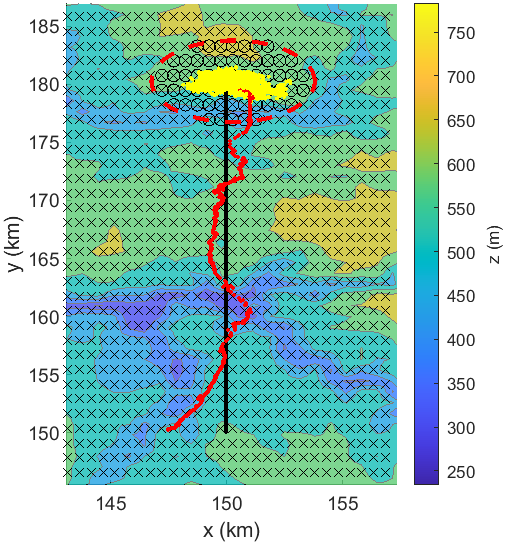
\includegraphics[width=\textwidth]{../../Images/Trajectoire FUSION 2024.png}
\end{center}
\end{column}

\begin{column}{0.55\textwidth}
\begin{center}
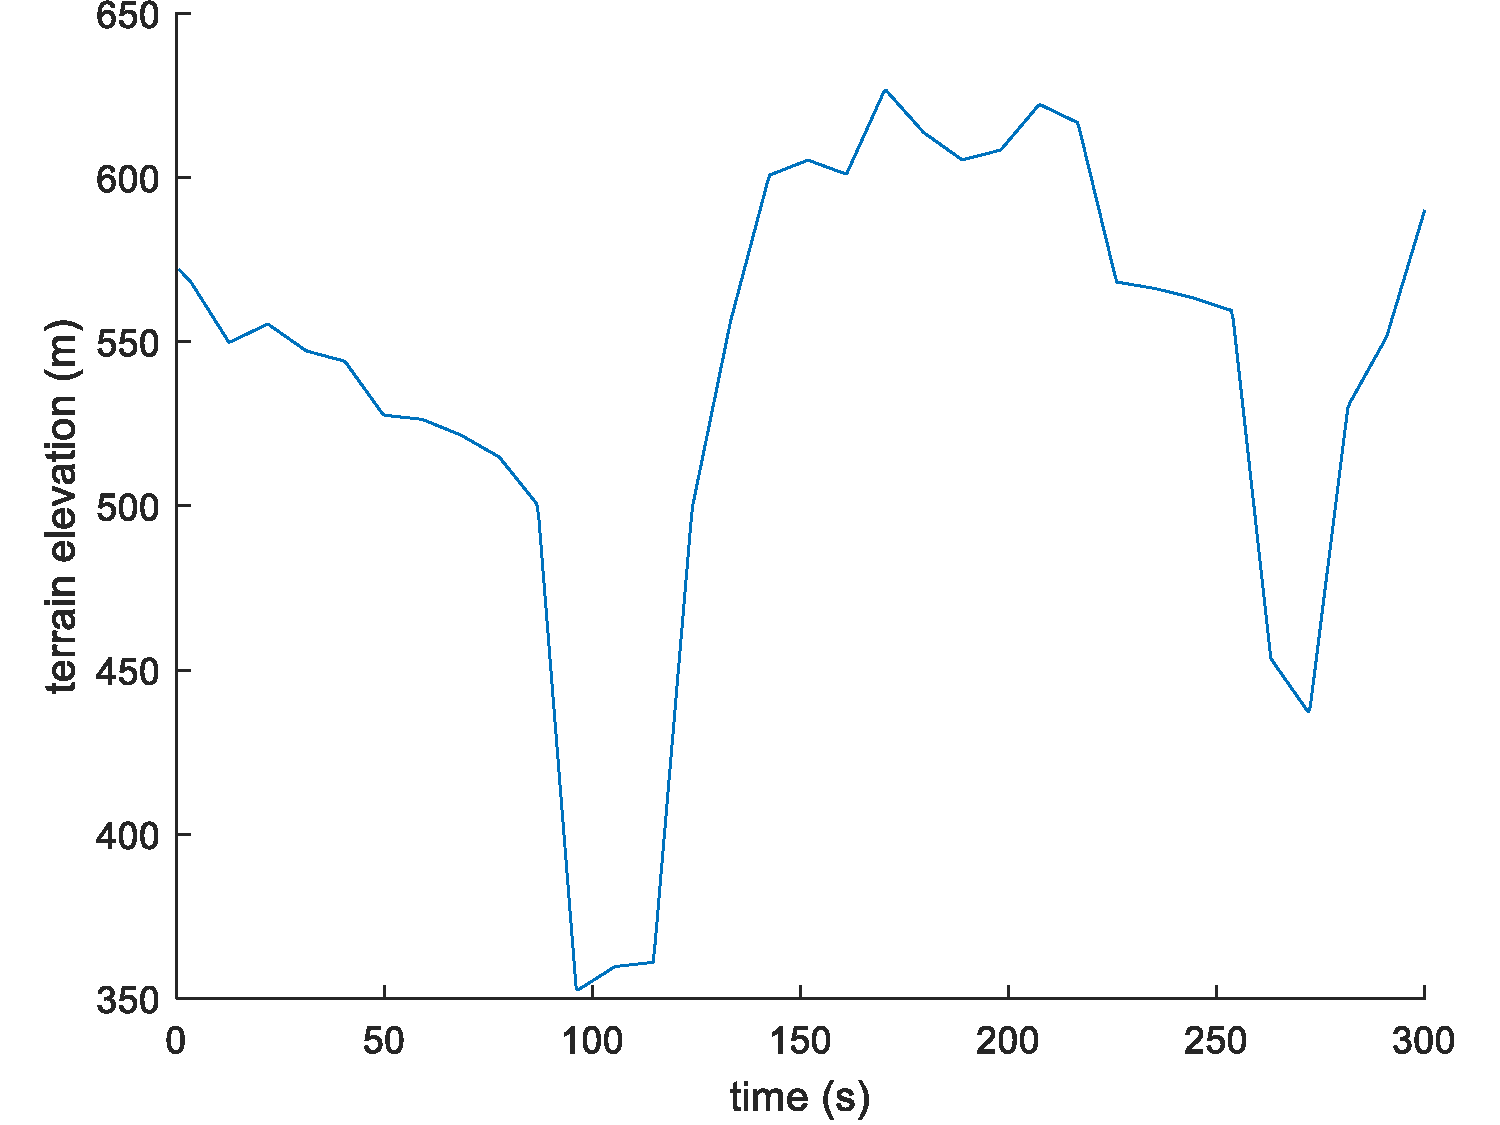
\includegraphics[width=\textwidth]{../../Images/Élévation de terrain FUSION 2024.pdf}
\end{center}
\end{column}

\end{columns}
\end{frame}

\begin{frame}{Numerical results}
\begin{block}{Comparison between AK-RPF and RPF}

\begin{center}
\renewcommand{\arraystretch}{1.1}
\begin{tabular}{|c|c|c|c|c|} \hline
\multirow{2}{*}{Resolution} & \multicolumn{2}{|c|}{RPF} & \multicolumn{2}{|c|}{AK-RPF} \\ \cline{2-5}
& Convergence & Final RMSE & Convergence & Final RMSE \\ \hlinewd{1.2pt}
0.40km & 92\% & 0.97km & / & / \\ \hline
0.70km & 34\% & 1.31km & / & / \\ \hline
0.78km & 21\% & 1.61km & / & / \\ \hline
0.88km & 3\% & 3.91km & 97\% & 0.43km \\ \hline
1.00km & 0\% & N/A & 81\% & 1.08km \\ \hline
1.17km & 0\% & N/A & 72\% & 1.15km \\ \hline
1.40km & / & / & 55\% & 1.19km \\ \hline
1.75km & / & / & 26\% & 2.35km \\ \hline
2.33km & / & / & 1\% & 2.24km \\ \hline
3.50km & / & / & 0\% & N/A \\ \hline
\end{tabular}
\end{center}

\end{block}
\end{frame}

\begin{frame}{Conclusion and future work}

\begin{block}{Our work}
\begin{itemize}
\item Dynamical reconstruction of the measurement function in a poorly-known environment
\item Comparison with a multi-linear interpolation-based RPF in a TAN scenario
\item[$\Rightarrow$] the AK-RPF is much more resilient to extreme scarcity of information
\end{itemize}
\end{block}

\begin{block}{Perspectives}
\begin{itemize}
\item More simulation scenarios
\item Gram matrix inversion at each step $\rightarrow$ computational heavy
\begin{itemize}
\item Particle clustering
\item Reduced-rank approximations
\end{itemize}
\end{itemize}
\end{block}

\end{frame}

\section{}
\miniframesoff

\begin{frame}{RMSE as a function of time}
\begin{center}
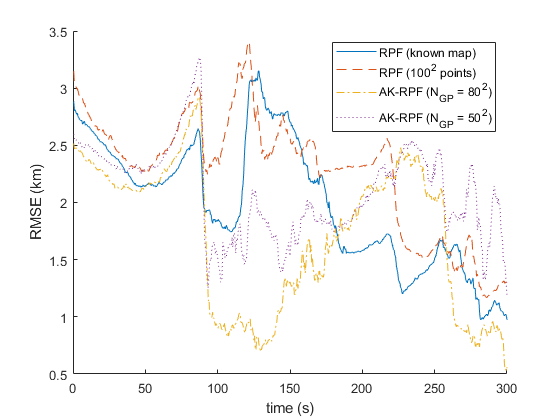
\includegraphics[width=0.9\textwidth]{../../Images/RMSEs FUSION 2024.png}
\end{center}
\end{frame}


\end{document}